\documentclass[tcc,capa]{texufpel}

\usepackage[utf8]{inputenc} % acentuacao
\usepackage{graphicx} % para inserir figuras
\usepackage[T1]{fontenc}

\hypersetup{
    hidelinks, % Remove coloração e caixas
    unicode=true,   %Permite acentuação no bookmark
    linktoc=all %Habilita link no nome e página do sumário
}

\unidade{Centro de Desenvolvimento Tecnológico}
\curso{Ciência da Computação}
\nomecurso{Bacharelado em Ciência da Computação}
\titulocurso{Bacharel em Ciência da Computação}

\unidadeeng{Technology Development Center}
\cursoeng{Computer Science}


\title{Visual Sims: uma ferramenta que utiliza Computação Gráfica para auxiliar a aprendizagem}

\author{Sampaio}{Letícia}
\advisor[Prof.~Dr.]{Torchelsen}{Rafael Piccin}
% \coadvisor[Prof.~Dr.]{Aguiar}{Marilton Sanchotene de}
% \collaborator[Prof.~Dr.]{Aguiar}{Marilton Sanchotene de}

%Palavras-chave em PT_BR
\keyword{Computação Gráfica}
\keyword{WebGL}
\keyword{Simulação}
\keyword{Interatividade}

%Palavras-chave em EN_US
\keywordeng{Graphyc Computing}
\keywordeng{WebGL}
\keywordeng{Simulation}
\keywordeng{Interactivity}

\begin{document}

% \renewcommand{\advisorname}{Orientadora}           %descomente caso tenhas orientadora
%\renewcommand{\coadvisorname}{Coorientadora}      %descomente caso tenhas coorientadora

\maketitle 

\sloppy

\fichacatalografica

%\folhadeaprovacao

%Composição da Banca Examinadora
\begin{aprovacao}{18 de junho de 2021} %data da banca por extenso
\noindent Prof. Dr. Rafael Piccin Torchelsen (orientador)\\
Doutor em Ciência da Computação pela Universidade Federal do Rio Grande do Sul.\\[1cm]

\noindent Prof. Dr. Marilton Sanchotene de Aguiar\\
Doutor em Ciência da Computação pela Universidade Federal do Rio Grande do Sul.\\[1cm]

\noindent Profa. Dra. Tatiana Aires Tavares\\
Doutora em Engenharia Elétrica pela Universidade Federal do Rio Grande do Norte.\\[1cm]

\end{aprovacao}

%Opcional
\begin{dedicatoria}
  Gostaria de dedicar este trabalho à comunidade discente dos cursos de Ciência e Engenharia da Computação. Este trabalho é acima de tudo, para a comunidade.
\end{dedicatoria}

%Opcional
\begin{agradecimentos}
  Agradeço primeiramente a minha família, por ter me incentivado a procurar um curso superior e me proporcionar esta experiência. 
  À minha namorada, que me mostrou a importância de se dedicar a tudo que fazemos, sempre dando o nosso melhor.
  Por fim, agradeço ao meu orientador, que continuou trabalhando comigo apesar dos prazos que impus a ele.
\end{agradecimentos}

%Opcional
\begin{epigrafe}
  It's not stupid if it works.\\
  {\sc --- Alunos de computação}
\end{epigrafe}

%Resumo em Portugues (no maximo 500 palavras)
\begin{abstract}
Para alunos dos cursos de Ciência e Engenharia de Computação encontrar conteúdo para estudar é uma tarefa fácil, entretanto existem poucas fontes de pesquisa que disponibilizam um conteúdo interativo. Conceitos ensinados de forma apenas teórica podem surgir como barreira para uma parcela desses alunos, por isso transformar um conteúdo teórico em prático e tornar esse conteúdo acessível é o objetivo deste trabalho. Este trabalho propõe o desenvolvimento de uma plataforma web, aberta a contribuições, com exemplos visuais e interativos de conteúdos abordados nas disciplinas de graduação dos cursos de Ciência e Engenharia de Computação. Utilizando conceitos de computação gráfica o aluno poderá visualizar exemplos e aprender de forma mais fácil o conteúdo abordado. Além da versão visual também será disponibilizado uma explicação textual do conteúdo. O site poderá dessa forma ser utilizado como ferramenta para estudo extra classe ou até como uma ferramenta para auxiliar o professor no ensino a distância.
\end{abstract}

%Resumo em Inglês (no maximo 500 palavras)
\begin{englishabstract}{Visual Sims: using Graphic Computing in a platform to help education}
For the students of Computer Science and Engineering, find content to improve studies it's easy, but there is a lack of interactive content. The main goal for this work is to give the students a platform where they can see a theoretical content in a more dynamical way. Besides the 3D experience, the student can also find the theoretical explanaition. These tipes of application give the student the power to learn in their own peace, which helps the fixation of the knowledge. The platform also aims to help professors, by giving them the support to create their own simulations, this way they can show the application of the themes beeing taught.
\end{englishabstract}

%Lista de Figuras
\listoffigures

%Lista de Tabelas
%\listoftables

%lista de abreviaturas e siglas
\begin{listofabbrv}{ABNT}%coloque aqui a maior sigla para ajustar a distância
        \item[ABNT] Associação Brasileira de Normas Técnicas
        \item[V-Sync] Vertical Synchronization
        \item[WebGL] Web Graphics Library
        \item[OpenGL] Open Graphics Library
        \item[API] Application Programming Interface
        \item[HTML] HyperText Markup Language
        \item[CSS] Cascading Style Sheets
\end{listofabbrv}

%Sumario
\tableofcontents

\chapter{Introdução}
\label{cap: introducao}

Trabalhar com ensino é uma além de passar o conhecimento aos alunos, estar sempre se desafiando e procurando novas formas de ensinar. Assim como a Computação é uma área em constante evolução, novas tecnologias são criadas e devemos nos manter atualizados no que pode nos ajudar e melhorar ainda mais nosso desempenho como profissionais. 

Cada vez mais o mundo virtual invade nossas vidas, já é esperado de nós que o tempo online seja maior que o offline. Além de ser uma grande ferramenta para o ensino, usar a tecnologia para é cada vez mais importante para manter o interesse dos alunos. 

Disciplinas disponíveis na grade curricular dos cursos de Ciência e Engenharia de Computação podem apresentar um nível alto de complexidade no seu conteúdo. A dificuldade enfrentada pelos alunos se associa ao estilo de ensino da disciplina, conteúdos teóricos têm a tendência de serem considerados mais difícil entre os estudantes. Esta barreira acarreta em uma perda de interesse por parte do aluno, nestes casos o professor pode buscar formas diferentes de atrair a atenção do aluno.

Outro desafio no aprendizado em Computação é a falta de uma infraestrutura que possibilite o aprendizado. Como apontado por~\cite{rauen2003abordagem} em sua pesquisa sobre o ensino de Redes de Computadores, a falta de laboratórios é um dos maiores agravantes para o aprendizado do conteúdo. Entretanto esse cenário não é comum somente ao ensino de Redes, para ensinar  Computação um laboratório bem equipado faz o nível de aprendizado dos alunos crescer.

Jogos demonstram ser uma ferramenta muito atrativa ao ensino~\cite{klawe1999computer}, por serem ferramentas visuais é possível transformar em um conceito teórico em uma aplicação lúdica. Porém, a criação de um jogo demanda maior dedicação ao seu desenvolvimento, por isso a proposta de simulações sobre conceitos pontuais parece mais promissor. Com elas é possível criar qualquer tipo de situação que facilite a exemplificação de um conceito, sem limitação de espaço ou casualidade de um evento acontecer. 

\section{Objetivos}

O presente trabalho tem como objetivo construir uma plataforma que funciona como galeria para simulações que auxiliem o ensino de conteúdos ligados a Computação. Como parte do objetivo, as simulações devem utilizar elementos gráficos e interativos para ajudar na compreensão, além de ser disponibilizado de forma gratuita e de fácil acesso aos alunos de Ciência e Engenharia de Computação.

\section{Organização do trabalho}

Este trabalho apresenta, no capítulo~\ref{cap: fundamentacao_teorica}, uma breve análise sobre as dificuldades encontradas no ensino, com foco no ensino de Computação. O capítulo~\ref{cap: trabalhos_relacionados} é dedicado aos trabalhos relacionados ao objetivo proposto, bem como métodos que outros autores encontraram. Uma breve navegação pelo site desenvolvido está disponível no capítulo~\ref{cap: navegacao}. No capítulo~\ref{cap: desenvolvimento} é apresentado a coleta de dados e estruturação do projeto para o resultado final do site proposto. No capítulo~\ref{cap: resultados_e_discussoes} é discutido os resultados do trabalho desenvolvido e o capítulo~\ref{cap: conclusao} encerra este trabalho apresentando a conclusão e uma visão para o que pode ser o futuro deste trabalho.

\chapter{Fundamentação teórica}
\label{cap: fundamentacao_teorica}

Cada individuo tem a sua forma de aprender, bem como cada professor tem a sua forma de ensinar. Por este motivo é essencial que o estudante se prepare previamente e saiba a melhor forma de assimilar um novo conhecimento e que o professor esteja aberto aos diferentes tipos de alunos que vai encontrar. Entretanto, os estilos de ensino e aprendizado geralmente não são compatíveis~\cite{felder1988learning}.

Estas duas realidades têm o mesmo objetivo, solidificar o conhecimento do aluno para o desenvolvimento de um bom profissional. Então a busca por métodos inovativos de aprendizado é um tópico recorrente em diversas áreas, não só ligadas à Computação, mas sempre com o intuito de tornar o conhecimento mais adaptável a realidade do estudante e do professor. 

Entretanto, para encontrar uma ferramenta de auxilio, precisamos saber as necessidades que encontramos. 

\section{Formas de ensino}

Existem duas grande vertentes do ensino, o Ensino Presencial e o Ensino à Distância. Essas duas formas de passar o conhecimento possuem grandes diferenças e os seus desafios. 

\subsection{Ensino Presencial}

O Ensino Presencial consiste em aulas onde os professores passam o conteúdo aos alunos de forma verbal, em forma de palestra ou debate. Também é comum a apresentação de exemplos de aplicação da matéria proposta. Neste formato não é usual a apresentação de mídias em aula, este padrão é seguido por se acreditar que mídias possam fazer os alunos dispersarem e não passar o conteúdo da forma correta. Entretanto a boa utilização de exemplos visuais têm se mostrado mais apelativo aos olhos dos estudantes.

\subsection{Ensino Remoto}

No Ensino Remoto é comum a utilização de mídias para auxiliar no aprendizado, as próprias aulas são ministradas em ambientes virtuais. Portanto o uso de outras formas de apresentar o conteúdo já está intrínseco no formato remoto. A fixação do conteúdo geralmente se dá por meio de atividades e trabalhos e o aluno está mais inserido ao uso de tecnologias para resolver suas atividades.

Em ambos os âmbitos do ensino, exemplos do conteúdo que o aluno pode interagir e estimula a sua curiosidade têm demonstrado resultados melhores do que o ensino tradicional em cursos de graduação.

\section{Simulações no ensino}%não gostei do nome mas por enquanto fica

No contexto de cursos de Computação, é comum aos professores buscarem formas de atrair a atenção dos alunos por meio de exemplos e atividades práticas que sejam interessantes para eles, como jogos e a robótica. Neste contexto simulações podem se tornar outro modo de cativar o interesse dos alunos, por serem aplicáveis para alunos de qualquer nível ou idade, além de retirar a dependência de um ambiente físico para exemplificação de um conteúdo~\cite{kincaid2003simulation}.

Entretanto o uso de simulações não se limita ao campo da Computação, diversas áreas do ensino buscam nas simulações uma nova estratégia de ensino~\cite{barreto2014simulaccao}. Este tipo de abordagem demonstra que a inovação da forma de ensino está acontecendo graças ao uso da tecnologia.

\section{Computação no Ensino}

Guiados por professores, os alunos têm o objetivo de aprender o conteúdo definido a priori, já a forma que o conhecimento é passado ao aluno fica por responsabilidade do professor. Ferramentas para auxiliar o ensino ajudam neste processo de adaptar a aula aos alunos. Uma forma da computação auxiliar é criando sistemas de recomendações ~\cite{drachsler2015panorama} ~\cite{aguiar2018recomendacao}. Entretanto, este tipo de solução ainda deixa o poder e a responsabilidade sob a mão do professor.

Outra forma que a computação auxilia é trazer a tecnologia para facilitar o acesso às informações. Uma ferramenta que se mostra presente nesse pretexto é o Ambiente Virtual de Aprendizagem (AVA) que conforme Voss~\cite{Voss_Nunes_Herpich_Medina_2015} é um ambiente que aperfeiçoa a qualidade do ensino dos alunos, por meio de atividades além da sala de aula. Esta ferramenta auxilia principalmente os alunos, que podem ter acesso à toda informação básica que necessitam com facilidade.

Considerando o contexto do ensino à Computação, muitas disciplinas possuem conteúdos muito extensos e complexos para serem apresentados no tempo previso, muitas vezes é uma corrida contra o relógio. É nesses casos que a construção do conhecimento com a ajuda da tecnologia tem um maior apelo. Transformar o conteúdo estático e "chato" em algo dinâmico e potencialmente divertido é um dos maiores motivadores do trabalho proposto.

Como forma de aprendizado, recursos que explorem estímulos visuais se mostram mais eficientes no aprendizado, pois podem explorar de forma lúdica conceitos mais complexos~\cite{klawe1999computer}. Por este motivo o propósito do projeto proposto é fazer com que até as cadeiras que não possuem uma vertente prática possam utilizar de uma ferramenta dinâmica como auxiliar.

\chapter{Trabalhos Relacionados}
\label{cap: trabalhos_relacionados}

Com base em simulações visuais e interativas os alunos podem explorar o que os conteúdos teóricos podem representar. Alguns trabalhos semelhantes já foram desenvolvidos e apresentaram resultado positivo em outros públicos alvo. Um trabalho similar, mas voltado aos alunos de ensino médio, é o site PHET~\cite{phet_2002}. Ele conta com diversas simulações que envolvem física, matemática e química. No site é possível acessar a biblioteca de simulações e interagir com variáveis e ver uma animação representando a mudança que essas variáveis trazem. 

Também temos o livro Immersive Linear Algebra~\cite{strom2017immersive} que conta com modelos em 3D e iterativos que ajudam na fixação e compreensão do conteúdo explicado. Com os modelos disponíveis no livro é possível ver as alterações que as fórmulas implicam nos gráficos e assim entender de forma gradual sua função.

Podemos utilizar o site WebGL Fundamentals~\cite{webgl_2017} também como referência de que contando com exemplos visuais o conteúdo sendo explicado se fixa melhor. No site aprendemos como utilizar a ferramenta WebGL, com exemplos iterativos junto à explicação.

O trabalho desenvolvido por~\cite{costa2018incentivando}, mostra resultados positivos ao uso de simulações no ensino de Arquitetura de Computadores. No trabalho, Costa desenvolve um simulador do microprocessador Z-80 para auxiliar a fixação do conteúdo. Ele ainda desenvolve uma avaliação quantitativa para validar o uso do simulador. A pesquisa foi realizada antes e depois da utilização do simulador e o resultado foi um aumento de 8,3\% na média de acertos, validando a premissa de que simulações interativas ajudam na fixação do conteúdo.

Outra plataforma que demonstrou resultado positivo foi a SIN~\cite{SBIE1607}, responsável por unificar os trabalhos:  TBC-SO/Web~\cite{woodhull2000sistemas},  o  OS Simulator~\cite{gadelha2010simulator} e o IO Simulator~\cite{medeiros2011io}. Todos os trabalhos abordam temas do ensino da disciplina de Sistemas Operacionais. Os resultados do trabalho desenvolvido com base no SIN mostrou uma grande aprovação dos alunos que utilizaram a plataforma, também foi apontado pelos docentes o aumento da produtividade das aulas ministradas utilizando a plataforma.

Por fim temos o VisEdu-CG~\cite{montibeller2014visedu}, uma plataforma que auxilia o ensino na disciplina de Computação Gráfica. Na aplicação criada é possível interagir com o ambiente, posicionando novos objetos na cena e adicionando comandos e propriedades a eles. Um ponto importante apresentado no trabalho é a importância de fazer a aplicação com uma boa usabilidade, afim de não se tornar uma barreira para o aprendizado.

Os trabalhos relacionados apresentam principalmente a receptividade dos alunos com a inserção de simulações interativas no processo de aprendizado. Porém elas apresentam soluções pontuais para um publico alvo menor. A proposta deste trabalho tem como objetivo abranger todas as disciplinas dos cursos de Engenharia e Ciência da computação. 

\chapter{Navegação}
\label{cap: navegacao}

Antes de tratar sobre as tecnologias utilizadas é importante termos uma visão do que estamos falando, por isso a seguir serão apresentadas as telas e navegação da plataforma.

Ao abrir a plataforma o usuário já entra em contato com a proposta do site e elementos em 3D, visto na figura~\ref{home}. 

\begin{figure}[htbp]
  \centering 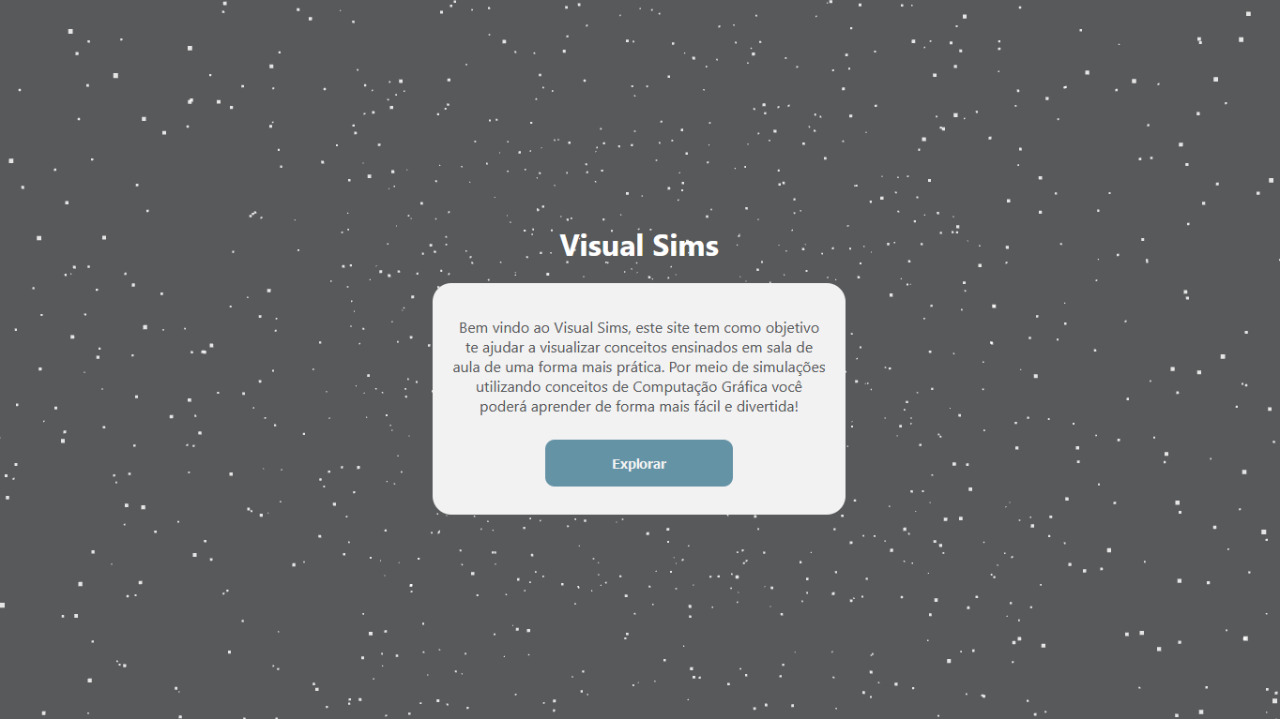
\includegraphics[scale=.2]{Navegacao/pagina_home.jpeg}
  \caption{Página principal}
  \label{home}
\end{figure}

Seguindo o fluxo o usuário entrará na galeria de simulações, figura~\ref{galeria}, onde poderá visualizar mais informações sobre a simulação clicando nela, figura~\ref{card_galeria}.

\begin{figure}[htbp]
  \centering 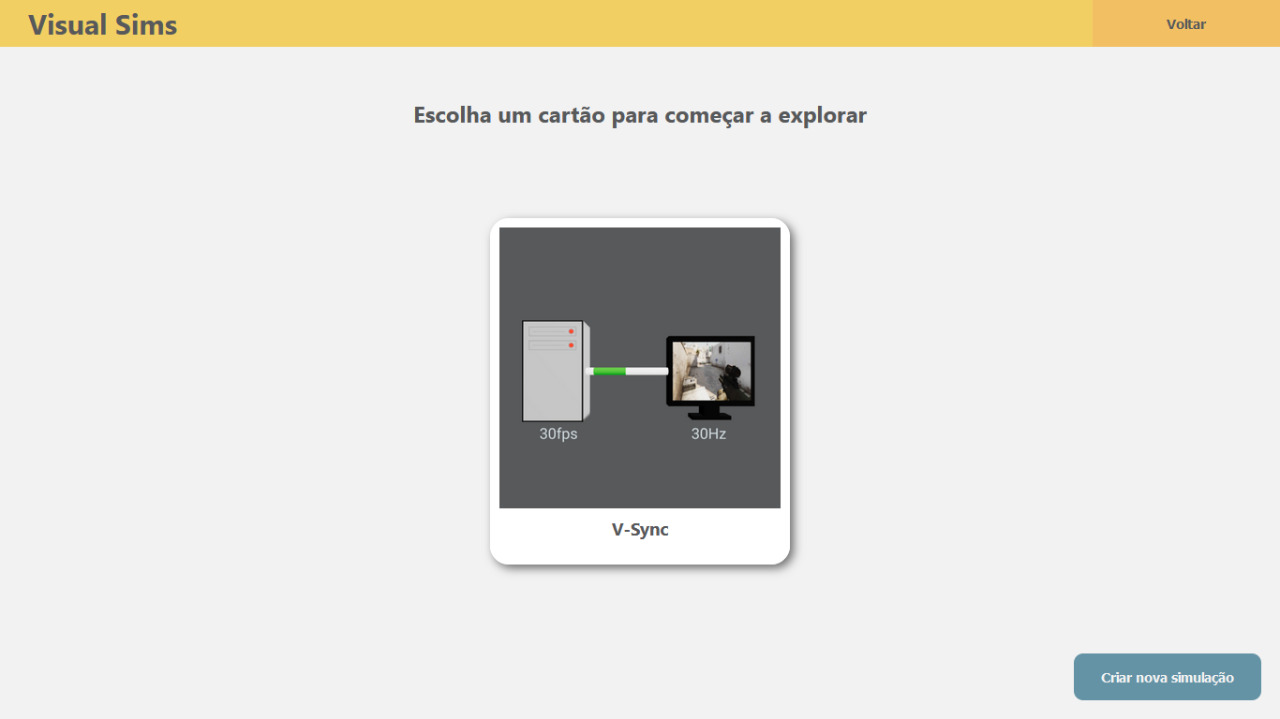
\includegraphics[scale=.2]{Navegacao/pagina_galeria.jpeg}
  \caption{Galeria de Simulações}
  \label{galeria}
\end{figure}

\begin{figure}[htbp]
  \centering 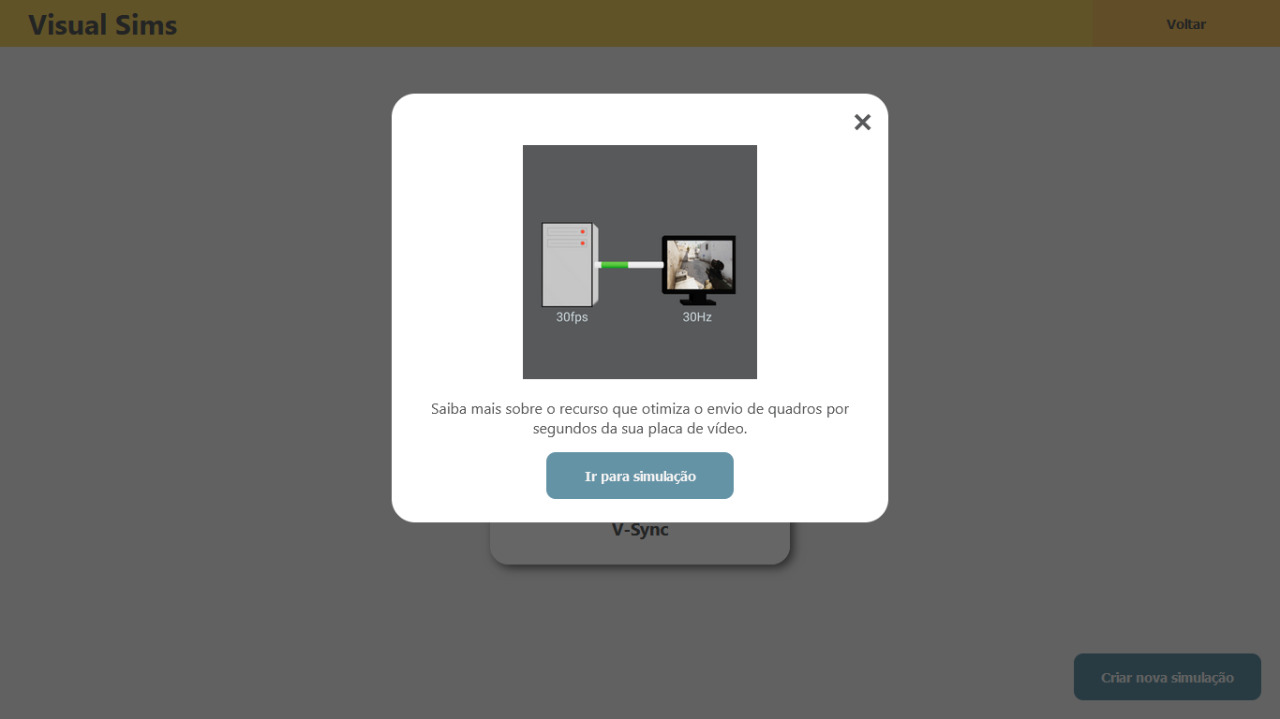
\includegraphics[scale=.2]{Navegacao/card_galeria.jpeg}
  \caption{Mais informações}
  \label{card_galeria}
\end{figure}

Após a escolha da simulação desejada o usuário é redirecionado para a página contendo o modelo da simulação, figura~\ref{simulacao}. Na página de simulação o usuário pode interagir com o ambiente, explorando o painel à direita que contém uma explicação sobre a simulação e os controles que fazem alterações na simulação para complementar a explicação. 

\begin{figure}[htbp]
  \centering 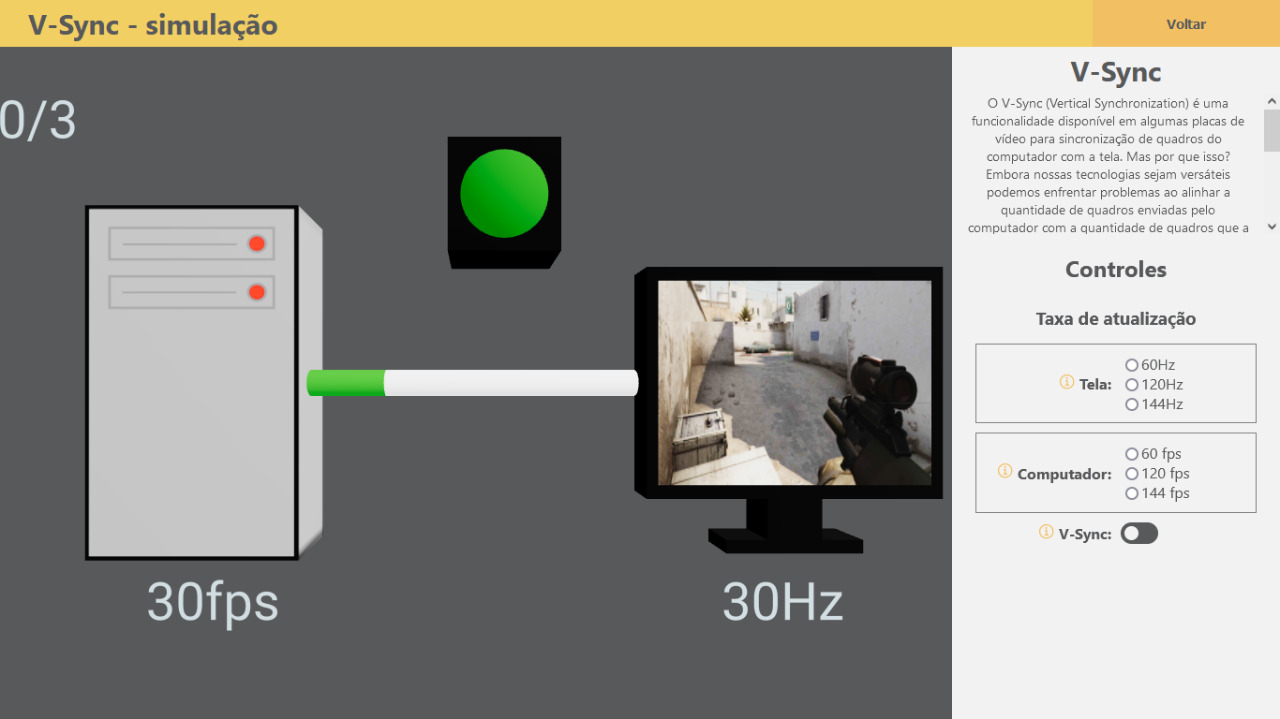
\includegraphics[scale=.2]{Navegacao/pagina_simulacao.jpeg}
  \caption{Simulação}
  \label{simulacao}
\end{figure}

As simulações não precisam ser controladas somente pelo painel, também é possível adicionar funcionalidades dentro da janela dos modelos 3D, como ao passar o mouse e aparecer mais informação sobre a simulação, figura~\ref{simulacao_extra}. 

\begin{figure}[htbp]
  \centering 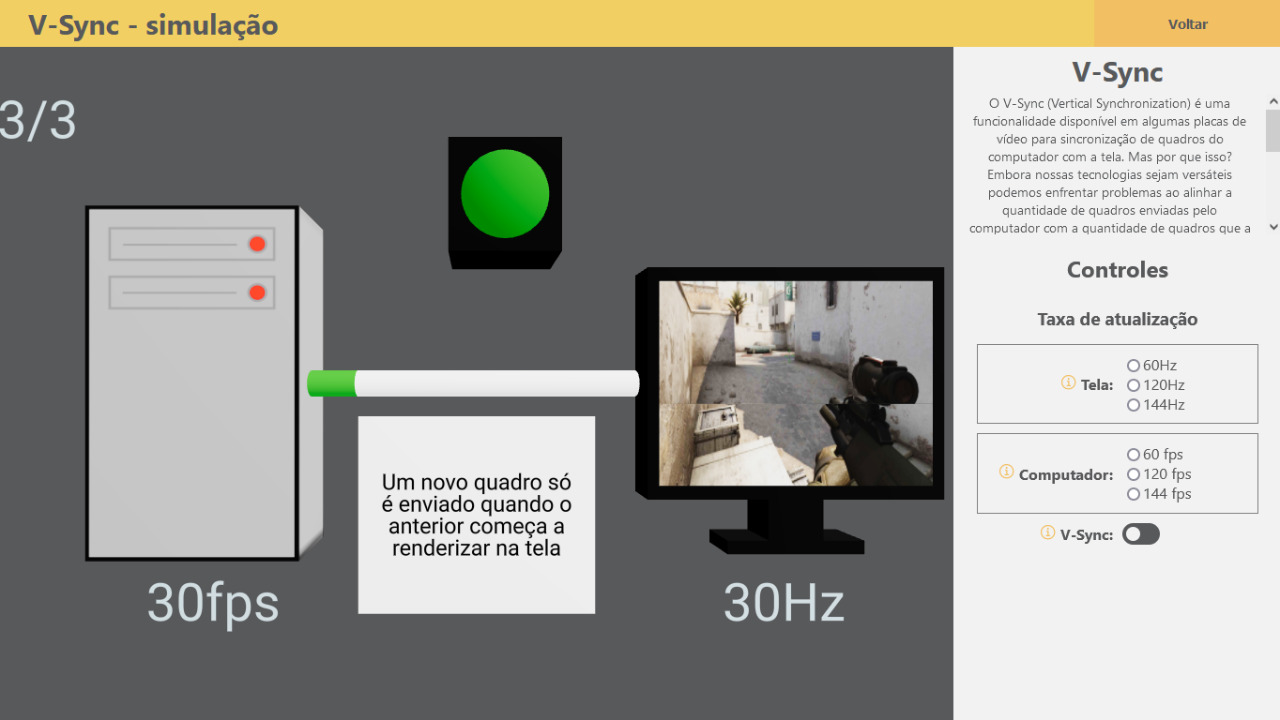
\includegraphics[scale=.2]{Navegacao/pagina_simulacao_extra.jpeg}
  \caption{Mais sobre a simulação}
  \label{simulacao_extra}
\end{figure}

\chapter{Desenvolvimento}
\label{cap: desenvolvimento}

Este capítulo é dedicado ao desenvolvimento da plataforma Visual Sims e uma breve discussão acerca das decisões que foram tomadas para o seu desenvolvimento. Abordando desde o levantamento dos dados necessários quanto as tecnologias utilizadas, apresentando suas vantagens frente ao projeto proposto.

A etapa de desenvolvimento teve como resultado um site desenvolvido para web, direcionado ao uso em desktop. A busca por informação deve ser livre, portanto uma plataforma web tem o potencial de atingir a maior parte do publico alvo. Outra vantagem deste tipo de aplicação é sua capacidade de criação, a tela do computador podendo ser comparada com uma tela em branco, em que tudo pode ser criado.

\section{Tecnologias}

O desenvolvimento de páginas estáticas tradicionais, com HTML e CSS, possibilitam a criação de diversos sites com diferentes propósitos, com a utilização da API WebGL as possibilidades de criação aumentam ainda mais. A combinação de JavaScript com WebGL criam uma ferramenta adaptável ao usuário da web.

Além de pensar na parte gráfica, é necessário levar em consideração a parte estrutural do projeto como um todo. Uma tecnologia que se mostrou bastante compatível com WebGL, e demonstrou ser bem estruturada, é a biblioteca React. Outra vantagem de escolher React é que por ser uma tecnologia bem atual é fácil de encontrar documentação e suporte na comunidade.

\subsection{WebGL}

WebGL é uma API em JavaScript que utiliza o elemento Canvas do HTML5 para renderização de elementos 2D e 3D. Esta API é uma evolução da API OpenGL, porém voltada ao desenvolvimento Web. Além de oferecer acesso a todos que possuem um browser compatível, essa tecnologia permite o acesso do navegador ao uso da GPU. Essa possibilidade aumenta a capacidade do que pode ser feito com WebGL.

Para entendermos melhor em que momento utilizamos o WebGL no processo de renderização, precisamos entender o fluxo de criação de um objeto em uma cena. Este processo é composto de diversas etapas, e muitas delas não necessitam de alterações. Na figura~\ref{pipeline_grafico} podemos ver o pipeline de renderização.

\begin{figure}[htbp]
  \centering 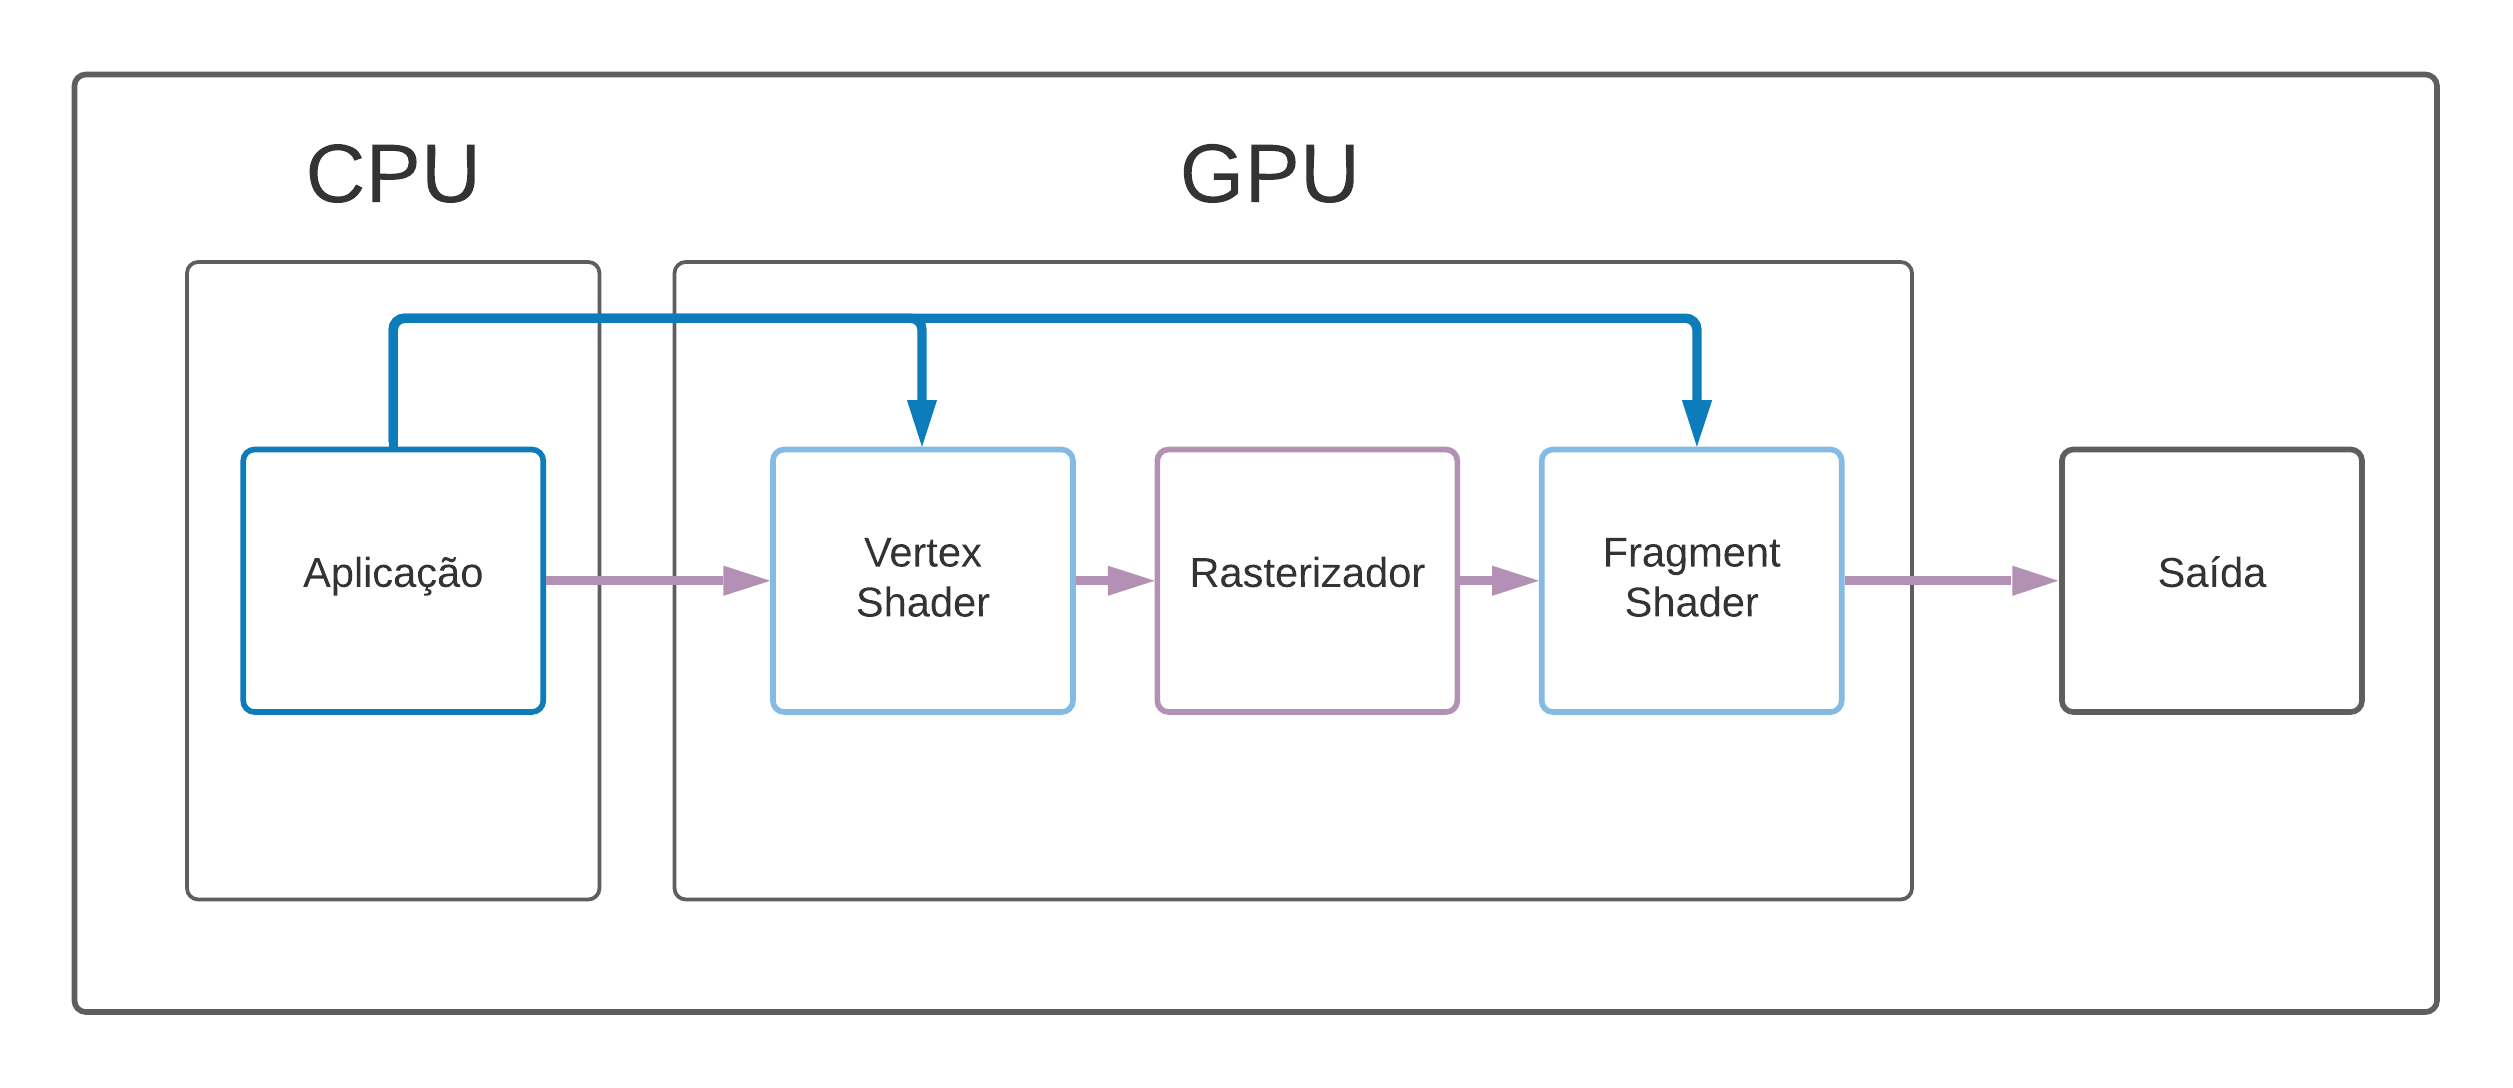
\includegraphics[scale=.7]{pipeline_grafico}
  \caption{Pipeline Gráfico}
  \label{pipeline_grafico}
\end{figure}% todo melhorar a imagem, colocar as outras etapas

Podemos observar destacado em azul as etapas que são programáveis. São elas que recebem o suporte do WebGL. As setas em roxo representam o fluxo de dados durante a execução do programa. Portanto, o WebGL fornece suporte para a criação do Vertex Shader, com a utilização da linguagem JavaScript, e o Fragment Shader, utilizando a linguagem GLSL. 

\subsection{React}

React é uma das bibliotecas para JavaScript mais utilizadas na criação de novos projetos web da atualidade. A sua popularidade se dá pela sua estrutura e reusabilidade. Dentro do React é possível criar estruturas modulares que serão reaproveitadas em diversas partes do projeto. 

Criando um componente como uma classe é possível chamar ela dentro de novos componentes e aproveitar tanto a parte funcional de JavaScript quanto o layout do componente construído com HTML. Entretanto essa não é a principal função do React. Se baseando no controle de estados, os Hooks, o React tem um alto controle do que está sendo renderizado na tela. Fazendo assim a integração com elementos gráficos algo mais trivial.

\subsection{Three.js}

Three.js é uma biblioteca que abstrai algumas declarações que precisaríamos fazer utilizando somente JavaScript e GLSL para programação em WebGL. 

\subsection{React Three Fiber}

React Three Fiber adiciona mais uma camada na comunicação entre a aplicação com React e a biblioteca Three.js. Ela permite a criação de componentes 3D reutilizáveis dentro da aplicação de forma mais alto nível.

\section{Coleta de dados}

Por se tratar de uma plataforma para exemplos de diversas disciplinas, foram considerados alguns modelos para serem produzidos e mostrar a capacidade da aplicação. Alguns dos modelos considerados foram: um modelo que mostra o envio de pacotes em uma rede de computadores e um sistema de controle de região crítica (mostrando como funciona a atomização das operações). No entanto, por termos mais exemplos voltados as cadeiras de Sistemas Operacionais e Redes de Computadores na literatura foi optado pela produção de uma simulação sobre o recurso V-Syc.

Após a decisão do modelo a ser desenvolvido se fez necessária uma pesquisa mais extensa sobre o que seria o recurso. A seguir irei aprofundar os conhecimentos sobre o recurso e falar sobre a vantagem de apresentar como conteúdo extra.

\subsection{V-Sync}

O V-Sync (Vertical Synchronization) é uma funcionalidade disponível nas placas de vídeo mais modernas para sincronização de quadros do computador com a tela. Embora nossas tecnologias sejam versáteis podemos enfrentar problemas ao alinhar a quantidade de quadros enviadas pelo computador com a quantidade de quadros que a tela recebe.

Essa diferença se torna um problema quando é possível ver uma quebra no quadro. Essa quebra ocorre porque a velocidade de renderização do quadro atual é diferente da velocidade em que os quadros estão chegando. Sendo a renderização ser feita de cima para baixo, enquanto um quadro está terminando de renderizar o próximo já inicia o processo, por isso acaba parecendo um corte na tela horizontalmente.

Para resolver este problema o V-Sync sincroniza o número de quadros enviados ao monitor de acordo com a sua capacidade, enviando um quadro somente quando o monitor estiver pronto para recebe-lo. Ao analisarmos o V-Sync também devemos levar em consideração que outros fatores podem atrasar o envio do quadro, como o processamento de cada quadro, e dessa forma parecer que o V-Sync na verdade faz baixar o fps. 

O conceito por trás do V-Sync traz ao aluno uma visão mais aprofundada sobre como a renderização funciona na prática. Por ser um conceito não abordado usualmente na sala de aula, esta simulação mostra a capacidade de ensinar algum conteúdo por meio de exemplos aplicados.


\section{Criação do Projeto}

Para o desenvolvimento do projeto, então, foi utilizada a combinação da biblioteca React juntamente com a React Three Fiber, para criar um projeto modular e reutilizável. Essas tecnologias trazem grande facilidade para o desenvolvimento, pois possuem uma estrutura de alto nível, possibilitando a criação de um código mais legível à novos desenvolvedores. Desta forma a curva de aprendizado da estrutura do projeto se torna menor.

Outra decisão de projeto importante é a forma de estruturação das pastas. Como em React o objetivo principal do projeto é criar componentes reutilizáveis, é ainda mais importante manter uma boa organização das pastas. Com isso em mente foi adotado para o projeto o Atomic Design. Que consiste em subdividir os componentes em Atomos, Moleculas e Organismos, dessa forma é fácil de encontrar os componentes desejados e de forma intuitiva criar novos componentes.

\subsection{Estrutura do projeto}

O Visual Sims é composto por um conjunto de componentes que servem de base para o desenvolvimento de uma nova simulação. A estrutura de pastas do projeto segue o Atomic Design, como já explicado, para a estrutura de pastas dos componentes. A figura~\ref{estrutura_de_pasta} mostra mais detalhadamente como estão estruturadas as principais pastas que um novo desenvolvedor irá utilizar.

\begin{figure}[htbp]
  \centering 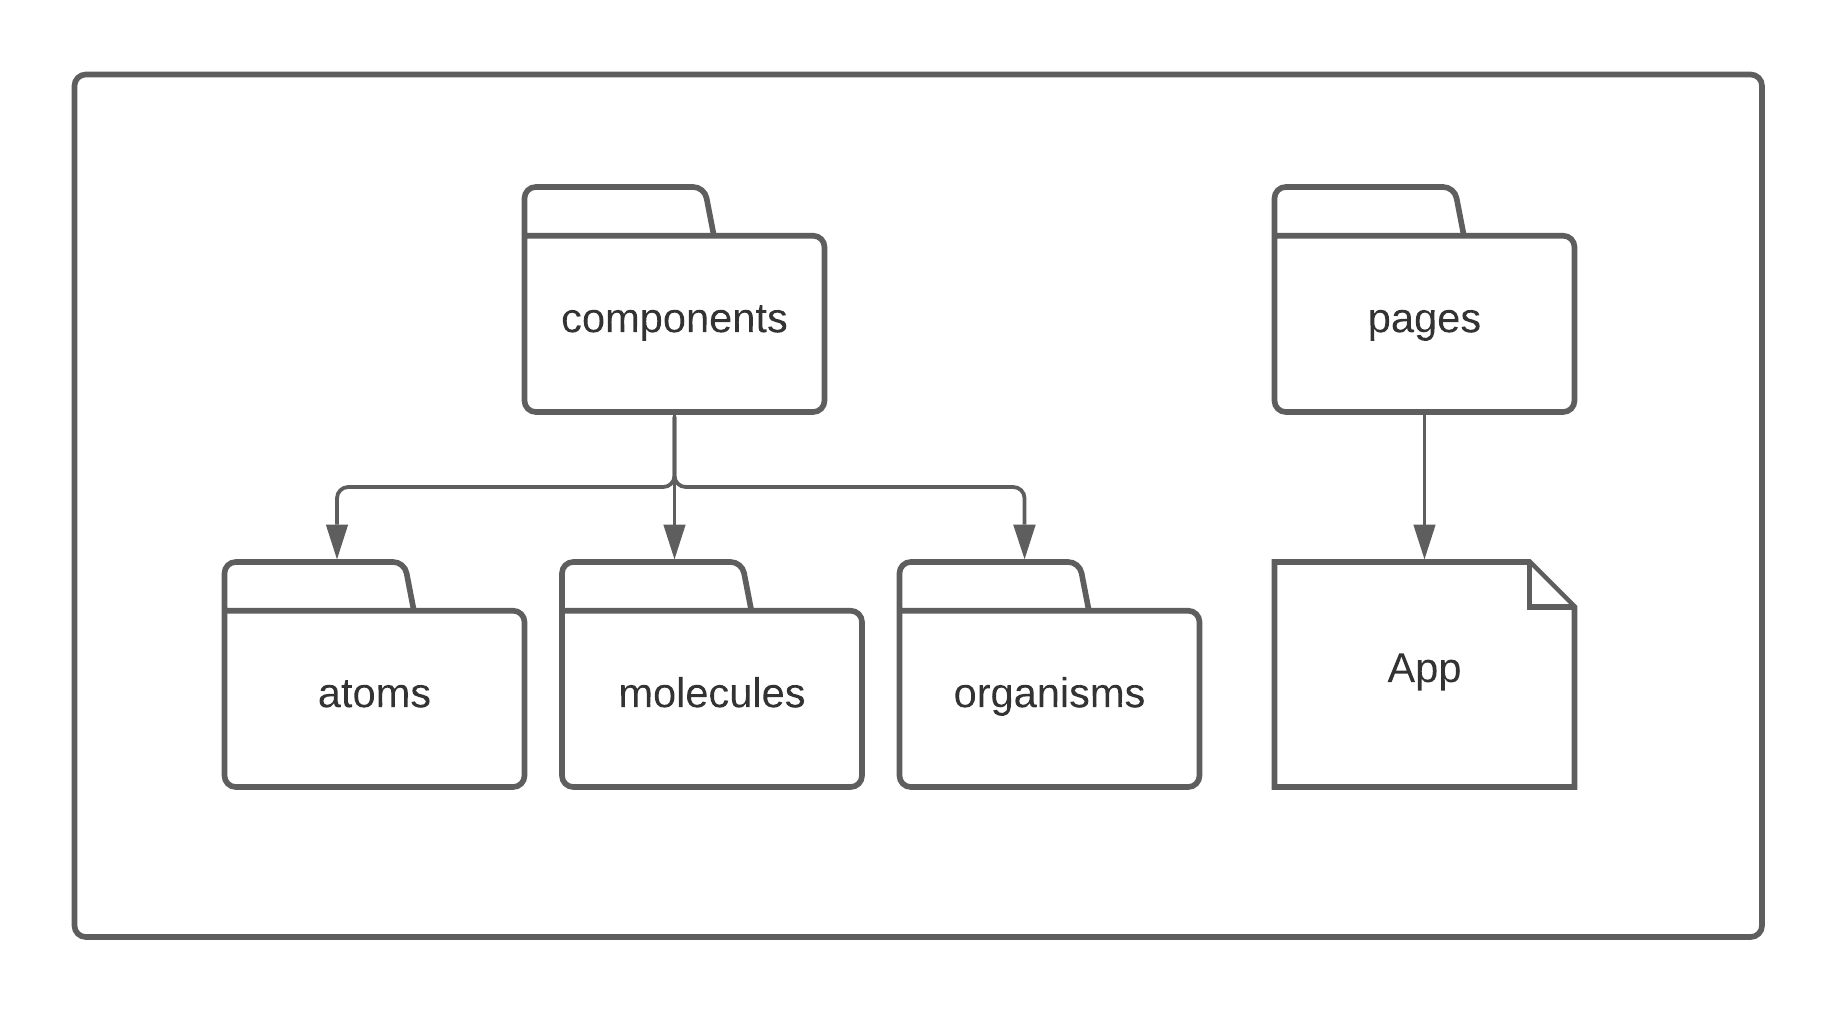
\includegraphics[scale=.7]{estrutura_de_pastas.png}
  \caption{Estrutura de Pastas}
  \label{estrutura_de_pastas}
\end{figure}

A pasta de átomos contém componentes pequenos e com pouca funcionalidade, tais como: padronização de botões e input, além de objetos 3D simples (caixas, cilindros, esferas). Assim criando a base para o desenvolvimento. Já as moléculas constituem de estruturas mais elaboradas, que lidam com átomos e o controle necessário sobre eles. O organismo representa o conjunto de moléculas e átomos.

Com o exemplo da simulação V-Sync, figura~\ref{pagina_simulacao_estrutura} podemos visualizar o item em vermelho como um átomo, os em azul como moléculas e a estrutura em verde, como um todo, um organismo.

\begin{figure}[htbp]
  \centering 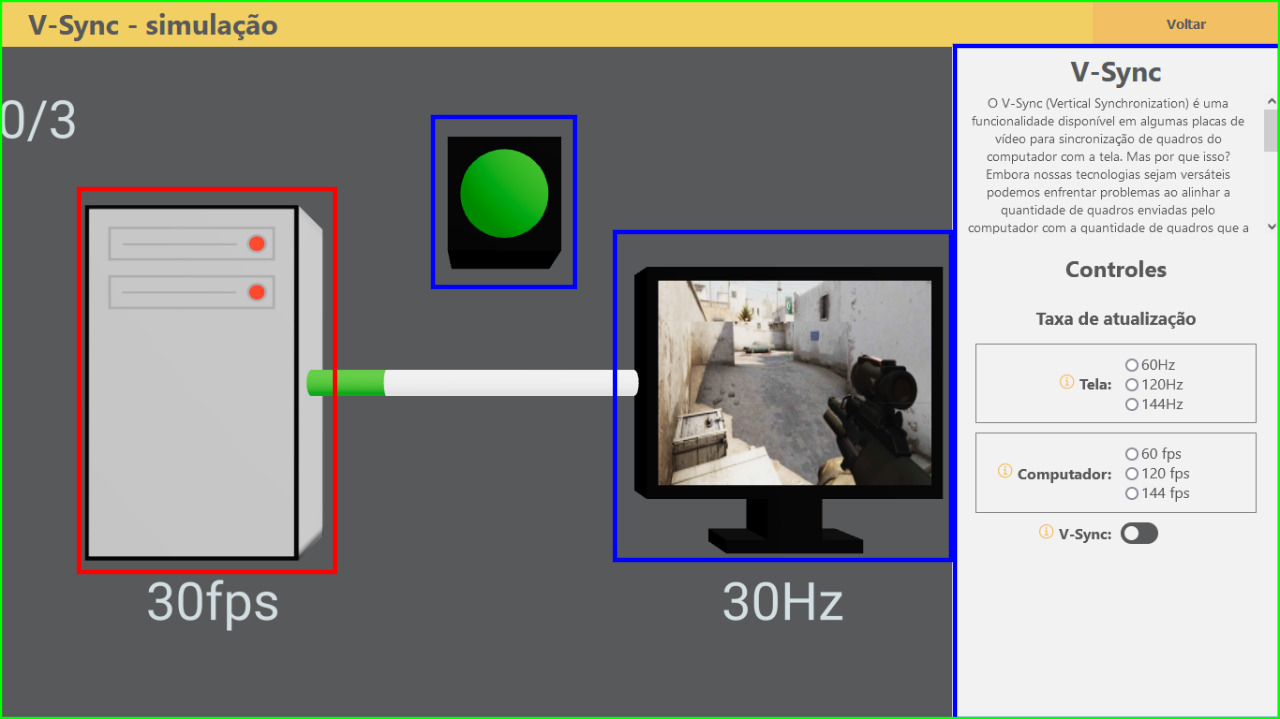
\includegraphics[scale=.3]{Navegacao/pagina_simulacao_estrutura.png}
  \caption{Estrutura da simulação V-Sync}
  \label{pagina_simulacao_estrutura}
\end{figure}

Desta forma o código se mantêm organizado e o desenvolvedor pode se concentrar melhor nos aspectos da sua simulação. 

\chapter{Resultados e Discussões}
\label{cap: resultados_e_discussoes}

A ideia inicial do projeto seria criar uma ferramenta dentro do site que permitisse a criação de novas simulações sem precisar realizar a programação do front-end. Infelizmente durante a fase de prototipação foram encontradas algumas dificuldades acerca de criar esta ferramenta dentro do prazo previsto. Um protótipo do que seria essa funcionalidade foi criado, figura~\ref{prototipo_criar_simulacao}. 

Sendo o foco do projeto criar uma plataforma que disponibilize exemplos visuais para auxiliar no ensino, o resultado está de acordo com o proposto. Por meio de utilização dos componentes e estruturas já criadas o desenvolvimento de uma nova simulação se dá de forma mais simples. O código está disponível e público para estudo e desenvolvimento.

\begin{figure}[htbp]
  \centering 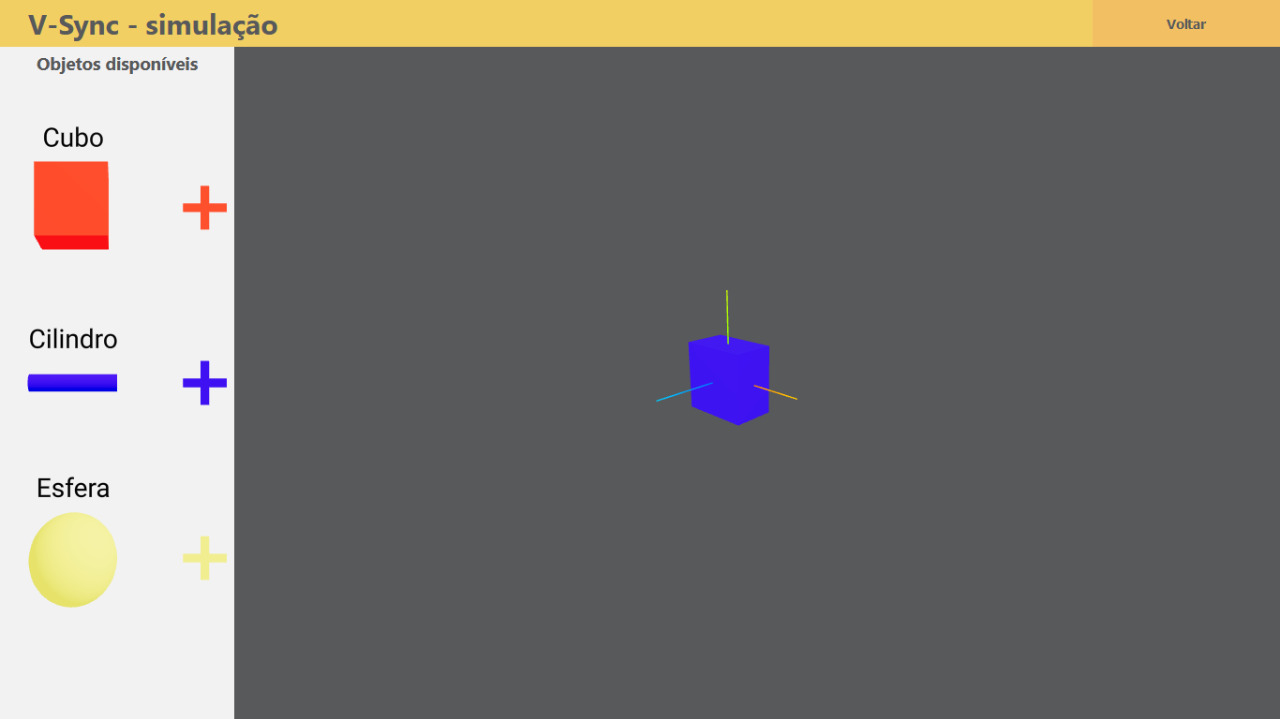
\includegraphics[scale=.2]{Navegacao/pagina_criar_simulacao.jpeg}
  \caption{Protótipo para criar simulação}
  \label{prototipo_criar_simulacao}
\end{figure}

Com base em pesquisas informais, foi constatado que o site oferece um resultado positivo, por meio de testes os usuários puderam aprimorar seus conhecimentos sobre o conteúdo apresentado. Foram levantados pontos de melhora em questão de de usabilidade, como para alguns não é possível ver a barra de rolagem do texto explicativo, figura~\ref{antes_texto_explicativo} e figura~\ref{melhoria_texto_explicativo} , por configuração de sistemas operacionais. Este tipo de avaliação demonstra que os usuários estavam envolvidos com a aplicação e também que a plataforma têm potencial para demonstrar o interesse deles.

\begin{figure}[htbp]
  \centering 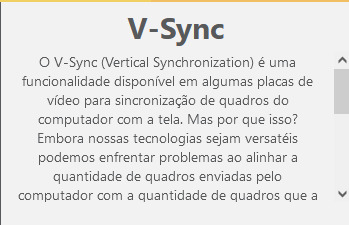
\includegraphics[scale=.3]{Navegacao/antes_texto_explicativo.jpeg}
  \caption{Texto explicativo antes da melhoria}
  \label{antes_texto_explicativo}
\end{figure}

\begin{figure}[htbp]
  \centering 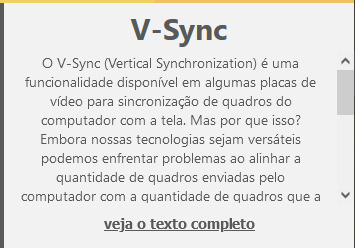
\includegraphics[scale=.3]{Navegacao/melhoria_texto_explicativo.jpeg}
  \caption{Texto explicativo após melhoria}
  \label{melhoria_texto_explicativo}
\end{figure}

\section{Formulário teste}

Para validar o trabalho final desenvolvido, foi realizada uma pesquisa abordando a funcionalidade da aplicação. Foi optado por um questionário curto para conferir se os usuários conseguiriam entender o propósito do site e avaliar a abordagem da simulação proposta. 

O formulário foi dividido em três partes, sendo a primeira antes do acesso ao site, a segunda um redirecionamento ao site e por ultimo algumas perguntas pós acesso ao site. O intuito desta pesquisa foi levantar possíveis melhorias ao site e a simulação apresentada. As questões do formulário podem ser encontradas no anexo~\ref{anexo: formulario}.

Quando perguntado aos participantes da pesquisa se, após o uso do simulador, entenderam o conceito explicado obtivemos o seguinte resultado: 

\begin{figure}[htbp]
  \centering 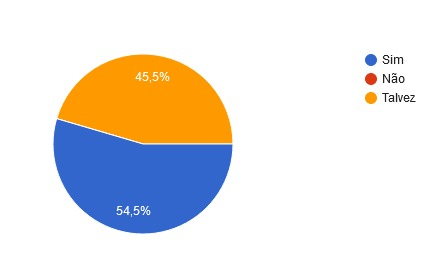
\includegraphics[scale=.3]{Graficos/resultado_compreendeu_simulacao.jpeg}
  \caption{Resultado: Você entendeu a explicação sobre V-Sync?}
  \label{resultado_compreendeu_simulacao}
\end{figure}

Este resultado se mostra promissor em conjunto com as respostas da questão seguinte, embora os participantes tenham respondido talvez, todos conseguiram desenvolver uma resposta satisfatória para explicar a funcionalidade do V-Sync.

As demais perguntas do formulário serviram para validação da funcionalidade o site e levantamento de possíveis problemas encontrados em diferentes sistemas operacionais e resoluções de telas. Um resultado levantado na pesquisa foi a demanda pelos usuários da criação de um ambiente voltado ao acesso pelo celular.

\chapter{Conclusão}
\label{cap: conclusao}

Este trabalho apresentou os resultados obtidos após o estudo e desenvolvimento da plataforma Visual-Sims. Considerando o contexto dos alunos de cursos de Computação, a plataforma fornece o suporte necessário para o desenvolvimento de novas simulações e a sua aplicação na sala de aula. 

Durante o desenvolvimento as dificuldades encontradas resultaram em uma nova abordagem sobre a plataforma, mas mesmo com as alterações o propósito se manteve. Ajudar a comunidade acadêmica, oferecendo uma ferramenta que auxilie o ensino, sempre foi o propósito do trabalho. 

Além do embasamento teórico e o desenvolvimento foi realizada uma pesquisa que mostrou a capacidade de aprendizado com as simulações. Esta pesquisa pode ser considerada como ponto de partida para trabalhos futuros. Um ponto a ser considerado é a melhoria na experiência de usuário, detalhes que algumas vezes podem deixar o usuário confuso. 

Como sugestão de trabalhos futuros podemos apontar o desenvolvimento de uma ferramenta de criação de simulação integrada a plataforma. Outra possibilidade é fazer a integração da plataforma com sistemas de análise de acesso, afim de descobrir a forma que os alunos interagem com as simulações e tornar elas mais efetivas.

Considerando a base do projeto criado, alindo os resultados obtidos e as indicações de melhorias é possível criar uma plataforma muito mais completa.

\bibliographystyle{abnt}
\bibliography{bibliografia} 

% Apêndices (Opcional) - Material produzido pelo autor
% \apendices
% \chapter{Um Apêndice}

Anexos (Opcional) - Material produzido por outro
\anexos
\chapter{Formulário proposto}
\label{anexo: formulario}

\section{Etapa 1}
1. Para começar, você sabe o que é V-Sync?
    1.1 - Sim
    1.2 - Não

2. Você poderia explicar o que é este recurso?

3. Você está matriculado em algum curso que envolva programação?
    1.1 - Sim
    1.2 - Não

\section{Etapa 2}

Link direcional ao site <https://leticiasampaio.github.io/visual-sims/>

\section{Etapa 3}

1. Você conseguiu acessar a simulação?
    1.1 - Sim
    1.2 - Não

2. Se a resposta anterior for não, por que não chegou à simulação?

3. Você entendeu o propósito do site?
    1.1 - Sim
    1.2 - Não
    1.3 - Talvez

4. Poderia explicar brevemente a função do site?

5. Você entendeu a explicação sobre V-Sync?
    1.1 - Sim
    1.2 - Não
    1.3 - Talvez

6. Poderia explicar o que entendeu da explicação?

7. Para qual finalidade você diria que o V-Sync é mais utilizado?

8. Você teria alguma sugestão de melhorias para o site?

9. Você estaria disposto(a) a participar de uma nova pesquisa com o site melhorado?
    1.1 - Sim
    1.2 - Não
    1.3 - Talvez


% \chapter{Outro Anexo}

% Faz a capa do CDROM
% \makecover

\end{document}

